%% Applied Soft Computing — Elsevier submission
%% Document class: elsarticle (standard Elsevier LaTeX template)
%% Compiled with: pdflatex -> bibtex -> pdflatex x2
%% Template version aligned with Elsevier Guide for Authors (2024)
%%
%% SUBMISSION CHECKLIST (Elsevier / Applied Soft Computing):
%%   [x] elsarticle document class
%%   [x] Highlights (3–5 bullets, ≤85 chars each)
%%   [x] Structured abstract
%%   [x] 6–8 Keywords
%%   [x] Numbered sections (no "Abstract" section number)
%%   [x] CRediT Author Statement
%%   [x] Declaration of Competing Interest
%%   [x] Data Availability Statement
%%   [x] Acknowledgements
%%   [x] Numbered reference list (Elsevier numeric style)
%%   [x] Scope alignment: Neural Networks, Hybrid Methods, Neurocomputing,
%%       Probabilistic Computing — explicitly stated throughout
%% ─────────────────────────────────────────────────────────────────────────────

\documentclass[review,12pt,authoryear]{elsarticle}
%% Options:
%%   review    = double-spaced, single column (for peer review)
%%   12pt      = font size
%%   authoryear= author–year citations (switch to 'number' if preferred)
%%
%% For final accepted version, change to:
%%   \documentclass[final,1p,times,twocolumn]{elsarticle}

%% ── Packages ─────────────────────────────────────────────────────────────────
\usepackage{amsmath,amssymb}
\usepackage{graphicx}
\usepackage{booktabs}
\usepackage{multirow}
\usepackage{tabularx}
\usepackage{xcolor}
\usepackage{hyperref}
\usepackage{microtype}
\usepackage{algorithm}
\usepackage{algpseudocode}
\usepackage{enumitem}
\usepackage{tikz}
\usetikzlibrary{arrows.meta, positioning, shapes.geometric, backgrounds, fit}
\usepackage{lineno}   % line numbers for review — remove for final
\modulolinenumbers[5]
\usepackage{caption}
\usepackage{subcaption}

\hypersetup{
  colorlinks=true,
  linkcolor=blue!60!black,
  citecolor=blue!60!black,
  urlcolor=blue!60!black
}

%% ── Macros ───────────────────────────────────────────────────────────────────
\newcommand{\todo}[1]{\textcolor{red}{\textbf{[TODO: #1]}}}
\newcommand{\modelname}{\textsc{ConceptAnchor}}
\newcommand{\dataset}{MIMIC-IV (v2.2)}
\newcommand{\eg}{\textit{e.g.,}\ }
\newcommand{\ie}{\textit{i.e.,}\ }

%% ── Journal ──────────────────────────────────────────────────────────────────
\journal{Applied Soft Computing}

%% ═════════════════════════════════════════════════════════════════════════════
\begin{document}
\linenumbers   % remove for final submission

%% ── Highlights ───────────────────────────────────────────────────────────────
%% Required by Applied Soft Computing: 3–5 bullets, maximum 85 characters each.
%% Submitted as a SEPARATE document titled "Highlights" during online submission.
%% Reproduced here for completeness.
\begin{highlights}
\item We propose \modelname, a hybrid neurocomputing framework for clinical prediction.
\item Mid-level concept abstractions are grounded in the Clinical Frailty Scale (CFS).
\item Specialist neural agents process distinct EHR modalities per frailty dimension.
\item Concept alignment loss enforces soft, probabilistic concept supervision.
\item Interpretability improves without degrading 30-day readmission prediction.
\end{highlights}

%% ── Front matter ─────────────────────────────────────────────────────────────
\begin{frontmatter}

\title{Concept-Anchored Abstraction for Transparent Clinical Prediction:\\ A Hybrid Neural Multi-Agent Framework Aligned to the Frailty Index}

%% Author block — use full given names (Elsevier requirement)
\author[inst1]{FirstName LastName\corref{cor1}}
\ead{corresponding@institution.edu}

\author[inst2]{FirstName LastName}
\ead{author2@institution2.edu}

\author[inst1,inst2]{FirstName LastName}
\ead{author3@institution.edu}

\cortext[cor1]{Corresponding author. Tel.: +XX-XXX-XXXXXXX.}

\affiliation[inst1]{organization={Department of Computer Science, Institution One},
             city={City},
             country={Country}}

\affiliation[inst2]{organization={School of Medicine, Institution Two},
             city={City},
             country={Country}}

%% ── Abstract ──────────────────────────────────────────────────────────────────
\begin{abstract}
Clinical prediction models frequently learn spurious statistical associations that lack grounding in medical reasoning and are susceptible to distributional shift.
We propose \modelname, a hybrid neurocomputing framework that introduces \emph{human-aligned conceptual abstractions} at explicitly defined intermediate layers of a deep learning pipeline for electronic health record (EHR) analysis.
Grounded in the Clinical Frailty Scale (CFS), the framework decomposes patient data into five clinically meaningful dimensions—nutritional status, cognitive function, mobility, comorbidity burden, and psychosocial factors—each processed by a specialised neural agent.
A top-level integration agent then aggregates these concept-aligned embeddings through a learned attention mechanism, producing a final readmission risk score that is both accurate and interpretable.
Concept alignment is enforced via a composite soft supervision loss that combines mean-squared error and binary cross-entropy terms, coupling intermediate representations to clinically derived proxy labels without requiring direct annotation of the frailty dimensions.
Experiments on the \dataset{} dataset for 30-day hospital readmission demonstrate that \modelname{} achieves \todo{AUROC = X.XX, F1 = X.XX} while improving per-dimension concept alignment scores by \todo{$\Delta$CAS = X.XX} relative to an unconstrained baseline.
These results demonstrate that incorporating soft, probabilistic concept constraints into the abstraction hierarchy of a neural network increases transparency while preserving predictive performance.
All performance claims are strictly bounded to the tested clinical dataset and task.
\end{abstract}

%% ── Keywords ──────────────────────────────────────────────────────────────────
%% Applied Soft Computing: 6–8 keywords, separated by \sep
\begin{keyword}
Concept bottleneck models \sep
Hybrid neurocomputing \sep
Clinical decision support \sep
Hospital readmission prediction \sep
Frailty index \sep
Electronic health records \sep
Multi-agent neural networks \sep
Interpretable machine learning
\end{keyword}

\end{frontmatter}

%% ═════════════════════════════════════════════════════════════════════════════
\section{Introduction}
\label{sec:intro}

Soft computing methodologies—including neural networks, fuzzy systems, evolutionary algorithms, and probabilistic reasoning—have emerged as powerful tools for solving complex, imprecision-laden real-world problems \citep{zadeh1994soft}.
Among the most pressing such problems is clinical prediction from electronic health records (EHRs): a domain characterised by high dimensionality, heterogeneous data modalities, temporal dependencies, and abundant missing values, all of which align naturally with soft computing's tolerance for imprecision and uncertainty.

Deep neural networks have demonstrated strong empirical performance on EHR-based clinical prediction tasks such as hospital readmission \citep{choi2016retain}, sepsis detection \citep{henry2015targeted}, and mortality prediction \citep{rajpurkar2017chexnet}.
However, these models typically operate as black boxes, learning latent representations without explicit alignment to clinical concepts.
As a result, they may exploit spurious correlations—statistical patterns that hold in the training distribution but lack meaningful conceptual grounding—leading to brittle performance under distributional shift \citep{subbaswamy2021evaluating} and generating little trust among clinical end-users \citep{rudin2019stop}.

Clinical reasoning, by contrast, is fundamentally concept-driven.
A clinician assessing readmission risk does not process raw laboratory values as opaque numerical features; rather, they abstract these into higher-level clinical constructs—frailty, organ dysfunction, social risk, cognitive decline—and integrate these constructs into a holistic judgement.
This structured, hierarchical reasoning provides both a predictive mechanism and an auditable rationale.

We argue that neural network architectures should mirror this concept-driven abstraction process.
To this end, we propose \modelname{} (\underline{Concept}-\underline{Anchor}ed Clinical Prediction), a hybrid soft computing framework that injects human-aligned conceptual features at defined abstraction steps within a multi-agent neural pipeline.
The framework is grounded in the Clinical Frailty Scale (CFS) \citep{rockwood2005frailty}, a validated clinical taxonomy that decomposes patient health into five interpretable dimensions.
Each dimension guides the specialisation of a dedicated neural agent, which processes the corresponding EHR modality and produces a concept-aligned embedding.
Soft probabilistic supervision—implemented through a composite loss function blending regression and binary cross-entropy terms—encourages these embeddings to encode clinically meaningful information without requiring complete, expert-annotated concept labels.
A top-level integration agent, operating analogously to a physician synthesising specialist referrals, combines the dimension-specific embeddings via learned attention to produce the final prediction.

\textbf{Soft computing alignment.}
\modelname{} is explicitly positioned as a hybrid neurocomputing system \citep{abraham2005hybrid}: it combines the representational power of deep neural networks with the interpretability afforded by symbolic, concept-based constraints.
The probabilistic concept supervision loss can be viewed as a soft constraint analogous to fuzzy membership functions, allowing intermediate representations to approach—but not be rigidly assigned to—concept targets.
This tolerance for imprecision in concept assignment is a defining characteristic of soft computing and is essential given the noisy, incomplete nature of EHR data.

\textbf{Contributions.} This paper makes the following contributions to applied soft computing and clinical AI:
\begin{enumerate}[leftmargin=*, label=\arabic*., noitemsep]
  \item \textbf{Framework}: \modelname, a hybrid neurocomputing framework for concept-anchored clinical prediction, applicable wherever structured clinical taxonomies exist.
  \item \textbf{Soft Concept Supervision}: A composite probabilistic loss function that enforces concept alignment without requiring complete annotation, combining continuous and binary supervision signals per dimension.
  \item \textbf{Frailty-Grounded Feature Design}: A principled mapping from raw \dataset{} modalities to the five CFS dimensions, providing a replicable blueprint for frailty-aligned EHR feature engineering.
  \item \textbf{Hierarchical Multi-Agent Architecture}: A modular neural architecture in which specialist agents and an integration agent mirror the structure of clinical multidisciplinary team consultation.
  \item \textbf{Empirical Evaluation}: Comprehensive experiments demonstrating the interpretability–performance trade-off on 30-day hospital readmission, including ablation studies and concept alignment quantification.
\end{enumerate}

The remainder of this paper is organised as follows.
Section~\ref{sec:related} reviews related work on soft computing for clinical prediction, concept-based models, and interpretable AI.
Section~\ref{sec:problem} formalises the problem.
Section~\ref{sec:method} presents the \modelname{} framework in detail.
Section~\ref{sec:experiments} describes the experimental setup.
Section~\ref{sec:results} reports and analyses results.
Section~\ref{sec:discussion} discusses implications, limitations, and ethical considerations.
Section~\ref{sec:conclusion} concludes.

%% ═════════════════════════════════════════════════════════════════════════════
\section{Related Work}
\label{sec:related}

\subsection{Soft Computing for Clinical Prediction}

Neural networks have been applied extensively to EHR-based clinical prediction \citep{choi2016retain, rasmy2021med}.
Recurrent architectures such as LSTMs and GRUs handle temporal dependencies in longitudinal patient records, while attention mechanisms selectively weight relevant time steps \citep{choi2016retain}.
Graph neural networks have been used to model comorbidity relationships encoded in diagnostic code ontologies \citep{shang2019pre}.
Beyond pure deep learning, hybrid approaches combining neural networks with rule-based systems, fuzzy logic, or evolutionary algorithms have demonstrated improved robustness and interpretability in healthcare applications \citep{abraham2005hybrid}.
Our work extends this tradition of hybrid soft computing by introducing a structured concept taxonomy as the organising principle of the hybrid architecture.

\subsection{Concept Bottleneck and Concept-Based Models}

Concept Bottleneck Models (CBMs) \citep{koh2020concept} route predictions through an intermediate layer of human-specified binary concept activations, enabling post-hoc intervention and providing an interpretable prediction pathway.
Extensions include Concept Embedding Models (CEMs) \citep{zarlenga2022concept}, which allow concepts to be encoded as continuous, high-dimensional embeddings rather than scalars, improving performance while retaining interpretability.
Sequential CBMs \citep{shin2023closer} model concept dependencies, while hybrid CBMs \citep{espinosa2022concept} blend learned and fixed concepts to handle incomplete concept annotations.
\modelname{} extends this line of work in three ways: (i) it operates on heterogeneous, multi-modal EHR data rather than image inputs; (ii) it employs soft probabilistic concept supervision rather than hard binary labels; and (iii) it uses a hierarchical multi-agent structure that mirrors the modular organisation of the clinical frailty taxonomy.

\subsection{Interpretable and Explainable AI in Healthcare}

Post-hoc explanation methods—SHAP \citep{lundberg2017unified}, LIME \citep{ribeiro2016should}, and attention visualisation \citep{choi2016retain}—are the dominant approach to EHR model interpretability.
However, their reliability as faithful explanations has been questioned: SHAP values can be sensitive to feature correlations \citep{kumar2020problems}, and attention weights do not necessarily reflect causal influence \citep{jain2019attention}.
Self-explaining models—which build interpretability into the forward pass—offer an alternative.
\modelname{} belongs to this family: interpretability is a structural property of the concept-anchored abstraction hierarchy, not a post-hoc approximation.

\subsection{Frailty Assessment with Machine Learning}

The frailty index has been operationalised in several machine learning models for readmission and mortality prediction \citep{segal2019frailty, stow2019predicting}.
These works typically treat frailty as a scalar covariable computed from deficit accumulation, feeding it as an engineered feature into otherwise standard models.
\modelname{} takes a fundamentally different approach: rather than computing frailty as a preprocessing step, it decomposes frailty into its constituent clinical dimensions and uses each dimension to guide a dedicated neural reasoning pathway, embedding frailty understanding into the model's computational graph.

\subsection{Multi-Agent Systems in Clinical AI}

Multi-agent architectures have been explored for clinical workflow modelling \citep{isern2010agents} and, more recently, for large-language-model-based medical question answering \citep{tang2023medagents}.
In the soft computing literature, multi-agent systems have been combined with fuzzy reasoning and neural networks to build distributed, robust decision support systems \citep{abraham2005hybrid}.
\modelname{} contributes a new instantiation of hybrid multi-agent neural systems in which agent specialisation is governed by a formal clinical taxonomy rather than ad hoc task decomposition.

%% ═════════════════════════════════════════════════════════════════════════════
\section{Problem Formulation}
\label{sec:problem}

Let $\mathcal{D} = \{(\mathbf{x}_i, y_i)\}_{i=1}^{N}$ denote the patient dataset, where $\mathbf{x}_i \in \mathcal{X}$ is a multimodal patient record and $y_i \in \{0,1\}$ indicates 30-day unplanned readmission.
Each record $\mathbf{x}_i$ comprises $M$ modality-specific inputs:
\begin{equation}
  \mathbf{x}_i = \left(\mathbf{x}_i^{\text{lab}},\, \mathbf{x}_i^{\text{vital}},\, \mathbf{x}_i^{\text{icd}},\, \mathbf{x}_i^{\text{med}},\, \mathbf{x}_i^{\text{note}}\right),
\end{equation}
corresponding to laboratory values, vital signs, ICD-10 diagnostic codes, medication records, and free-text clinical notes, respectively.

\textbf{Concept Set.}
Let $\mathcal{C} = \{c_k\}_{k=1}^{K}$ denote a set of $K$ clinically meaningful concepts grounded in the CFS taxonomy.
In our instantiation, $K = 5$ and $\mathcal{C}$ corresponds to:
\begin{equation}
  \mathcal{C} = \left\{c_{\text{Nut}},\, c_{\text{Cog}},\, c_{\text{Mob}},\, c_{\text{Com}},\, c_{\text{Psy}}\right\},
\end{equation}
for Nutritional, Cognitive, Mobility, Comorbidity, and Psychosocial dimensions.

\textbf{Objective.}
We seek a model $f: \mathcal{X} \to [0,1]$ that: (i) accurately predicts $y$ (\ie maximises AUROC), and (ii) routes its computation through intermediate concept representations $\mathbf{h} = (h_1, \ldots, h_K) \in \mathbb{R}^{K \times d}$ such that each $h_k$ is statistically aligned with concept $c_k$, as measured by a concept alignment score $\phi(h_k, c_k) \in [-1, 1]$.

\textbf{Soft Concept Labels.}
Rather than requiring binary concept annotations, \modelname{} uses clinically derived \emph{proxy labels} $\hat{c}_k^{(i)} \in \mathbb{R}$ that serve as soft supervision targets.
These proxies are computed from observable EHR features and approximate the underlying concept values with known noise.
This soft supervision paradigm is consistent with the fuzzy and probabilistic reasoning principles of soft computing, accommodating the inherent uncertainty in clinical concept operationalisation.

%% ═════════════════════════════════════════════════════════════════════════════
\section{Methodology: The \modelname{} Framework}
\label{sec:method}

\subsection{Architectural Overview}

Figure~\ref{fig:architecture} presents the \modelname{} architecture.
The framework comprises three computational tiers:

\begin{enumerate}[leftmargin=*, label=\arabic*., noitemsep]
  \item \textbf{Modality Encoders}: Modality-specific preprocessing and initial representation learning.
  \item \textbf{Specialist Concept Agents}: $K$ neural agents, each aligned to one CFS dimension, producing concept embeddings.
  \item \textbf{Integration Agent}: A top-level neural module that aggregates concept embeddings via learned attention to produce the final prediction.
\end{enumerate}

This three-tier structure is a hybrid neurocomputing system: the specialist agents implement distributed, parallel neural processing analogous to multi-agent systems in soft computing \citep{abraham2005hybrid}, while the concept alignment loss introduces a soft symbolic constraint layer that bridges sub-symbolic neural computation and symbolic clinical knowledge.

\begin{figure}[t]
  \centering
  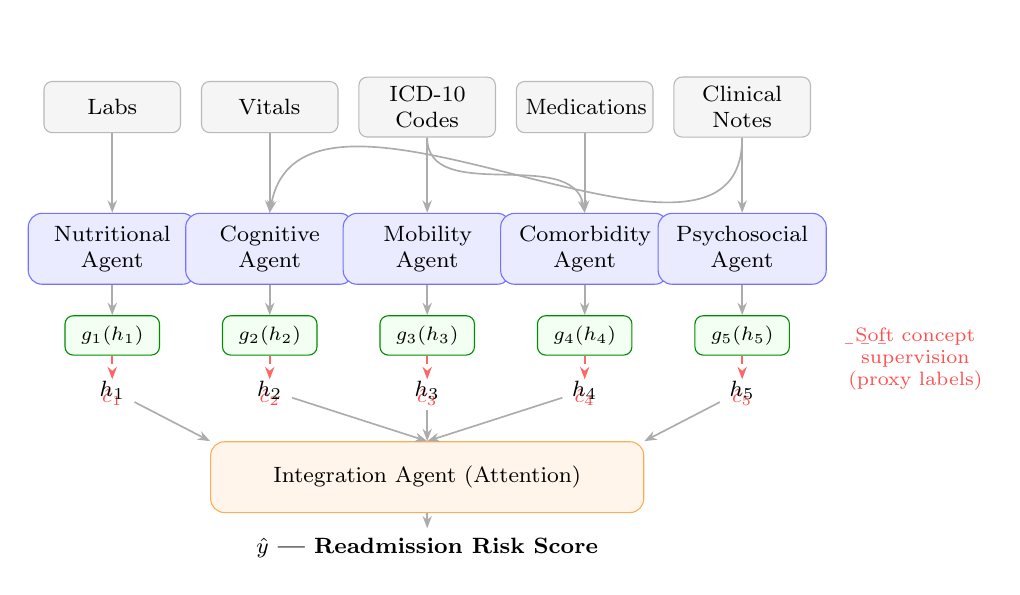
\begin{tikzpicture}[
    font=\small,
    agent/.style={rectangle, rounded corners=5pt, draw=blue!55, fill=blue!8,
                  minimum width=2.1cm, minimum height=0.9cm, align=center,
                  text width=1.9cm, font=\footnotesize},
    raw/.style={rectangle, rounded corners=3pt, draw=gray!55, fill=gray!8,
                minimum width=1.7cm, minimum height=0.65cm, align=center,
                text width=1.5cm, font=\footnotesize},
    integ/.style={rectangle, rounded corners=5pt, draw=orange!65, fill=orange!8,
                  minimum width=5.5cm, minimum height=0.9cm, align=center, font=\footnotesize},
    proj/.style={rectangle, rounded corners=3pt, draw=green!55!black, fill=green!5,
                 minimum width=1.2cm, minimum height=0.5cm, align=center, font=\scriptsize},
    arr/.style={-{Stealth[length=4.5pt]}, semithick, gray!65}
  ]
    %% ── Row 1: Raw modalities
    \node[raw] (lab)    at (0.0, 5.8)  {Labs};
    \node[raw] (vital)  at (2.0, 5.8)  {Vitals};
    \node[raw] (icd)    at (4.0, 5.8)  {ICD-10\\Codes};
    \node[raw] (med)    at (6.0, 5.8)  {Medications};
    \node[raw] (note)   at (8.0, 5.8)  {Clinical\\Notes};

    %% ── Row 2: Specialist Agents
    \node[agent] (a1) at (0.0, 4.0)  {Nutritional\\Agent};
    \node[agent] (a2) at (2.0, 4.0)  {Cognitive\\Agent};
    \node[agent] (a3) at (4.0, 4.0)  {Mobility\\Agent};
    \node[agent] (a4) at (6.0, 4.0)  {Comorbidity\\Agent};
    \node[agent] (a5) at (8.0, 4.0)  {Psychosocial\\Agent};

    %% ── Row 3: Concept embeddings + projection heads
    \node[proj] (p1) at (0.0, 2.9) {$g_1(h_1)$};
    \node[proj] (p2) at (2.0, 2.9) {$g_2(h_2)$};
    \node[proj] (p3) at (4.0, 2.9) {$g_3(h_3)$};
    \node[proj] (p4) at (6.0, 2.9) {$g_4(h_4)$};
    \node[proj] (p5) at (8.0, 2.9) {$g_5(h_5)$};

    %% Proxy label arrows (concept supervision)
    \foreach \n/\lab in {p1/$\hat{c}_1$, p2/$\hat{c}_2$, p3/$\hat{c}_3$, p4/$\hat{c}_4$, p5/$\hat{c}_5$} {
    }
    \draw[arr, dashed, red!60] (p1.south) -- ++(0,-0.3) node[below, font=\scriptsize, red!70]{$\hat{c}_1$};
    \draw[arr, dashed, red!60] (p2.south) -- ++(0,-0.3) node[below, font=\scriptsize, red!70]{$\hat{c}_2$};
    \draw[arr, dashed, red!60] (p3.south) -- ++(0,-0.3) node[below, font=\scriptsize, red!70]{$\hat{c}_3$};
    \draw[arr, dashed, red!60] (p4.south) -- ++(0,-0.3) node[below, font=\scriptsize, red!70]{$\hat{c}_4$};
    \draw[arr, dashed, red!60] (p5.south) -- ++(0,-0.3) node[below, font=\scriptsize, red!70]{$\hat{c}_5$};

    %% Concept embeddings
    \node[draw=none, font=\footnotesize] (h1) at (0.0, 2.2) {$h_1$};
    \node[draw=none, font=\footnotesize] (h2) at (2.0, 2.2) {$h_2$};
    \node[draw=none, font=\footnotesize] (h3) at (4.0, 2.2) {$h_3$};
    \node[draw=none, font=\footnotesize] (h4) at (6.0, 2.2) {$h_4$};
    \node[draw=none, font=\footnotesize] (h5) at (8.0, 2.2) {$h_5$};

    %% ── Row 4: Integration agent
    \node[integ] (integ) at (4.0, 1.1) {Integration Agent (Attention)};

    %% Output
    \node[draw=none, font=\footnotesize\bfseries] (out) at (4.0, 0.2)
          {$\hat{y}$ — Readmission Risk Score};

    %% Arrows: raw -> agents (with modality routing)
    \draw[arr] (lab)   -- (a1);
    \draw[arr] (vital) -- (a2);
    \draw[arr] (icd)   -- (a3);
    \draw[arr] (icd.south) to[out=270,in=100] (a4.north);
    \draw[arr] (med)   -- (a4);
    \draw[arr] (note)  -- (a5);
    \draw[arr] (note.south) to[out=270,in=80] (a2.north);

    %% Arrows: agents -> projection heads
    \draw[arr] (a1) -- (p1);
    \draw[arr] (a2) -- (p2);
    \draw[arr] (a3) -- (p3);
    \draw[arr] (a4) -- (p4);
    \draw[arr] (a5) -- (p5);

    %% Arrows: embeddings -> integration
    \draw[arr] (h1) -- (integ.north west);
    \draw[arr] (h2) -- (integ.north);
    \draw[arr] (h3) -- (integ.north);
    \draw[arr] (h4) -- (integ.north);
    \draw[arr] (h5) -- (integ.north east);

    %% Arrow: integration -> output
    \draw[arr] (integ) -- (out);

    %% Label: concept supervision
    \node[font=\scriptsize, red!70, align=center] at (10.2, 2.6)
          {Soft concept\\supervision\\(proxy labels)};
    \draw[red!50, dashed] (9.3, 2.8) -- (9.9, 2.8);

  \end{tikzpicture}
  \caption{\textbf{\modelname{} architecture.}
  Raw EHR modalities are routed to five specialist neural agents, each aligned to a CFS frailty dimension.
  Each agent produces a concept embedding $h_k$ and a projection $g_k(h_k)$ supervised by a soft proxy label $\hat{c}_k$ (red dashed arrows).
  The integration agent aggregates embeddings via learned attention to produce the final readmission risk score $\hat{y}$.}
  \label{fig:architecture}
\end{figure}

\subsection{Frailty Index as the Conceptual Anchor}

The Clinical Frailty Scale (CFS) \citep{rockwood2005frailty} is a validated nine-point ordinal scale that stratifies patients by accumulated health deficits.
We adopt the five underlying deficit domains of the CFS as the conceptual backbone of \modelname{} for three reasons:
\begin{enumerate}[leftmargin=*, label=(\roman*), noitemsep]
  \item Frailty is a validated predictor of hospital readmission independent of primary diagnosis \citep{stow2019predicting};
  \item Its five dimensions partition the space of patient health into non-overlapping, clinically interpretable domains;
  \item Each domain maps naturally to distinct EHR data modalities, enabling clean modality-to-agent routing.
\end{enumerate}

Table~\ref{tab:concept_mapping} details the mapping between CFS dimensions, EHR modalities, proxy labels, and clinical rationale.

\begin{table*}[t]
  \centering
  \caption{Mapping of CFS frailty dimensions to \dataset{} data modalities, proxy labels, and clinical rationale.
  Proxy labels marked with $\dagger$ are continuous; those marked with $\ddagger$ are binary.}
  \label{tab:concept_mapping}
  \begin{tabularx}{\textwidth}{lXXXX}
    \toprule
    \textbf{Dimension} & \textbf{Assigned Modalities} & \textbf{Key Features} & \textbf{Proxy Label $\hat{c}_k$} & \textbf{Clinical Rationale} \\
    \midrule
    Nutritional  & Labs, Vitals
      & Albumin, prealbumin, BMI, transferrin, weight change
      & \todo{Define proxy: e.g., serum albumin $<$ 3.5 g/dL or MUST score}$^\ddagger$
      & Malnutrition strongly predicts complications and readmission \citep{segal2019frailty} \\[4pt]
    Cognitive    & Clinical notes, Labs
      & Delirium ICD codes, MMSE proxy (NLP), ammonia, lactate
      & \todo{Define proxy: e.g., binary delirium flag from ICD-10 F05}$^\ddagger$
      & Cognitive impairment increases LOS, discharge complexity, and readmission risk \\[4pt]
    Mobility     & Vitals, ICD codes, Notes
      & Fall risk codes, PT/OT note presence, transfer-assist flags, gait speed proxy
      & \todo{Define proxy: e.g., ordinal mobility score from nursing notes NLP}$^\dagger$
      & Impaired mobility is a core frailty deficit and predictor of 30-day readmission \\[4pt]
    Comorbidity  & ICD codes, Medications
      & Charlson Comorbidity Index, polypharmacy count, Elixhauser score
      & Charlson Comorbidity Index$^\dagger$ (computed from ICD codes)
      & Multimorbidity and polypharmacy are primary drivers of readmission \citep{stow2019predicting} \\[4pt]
    Psychosocial & Clinical notes, ICD codes
      & Depression/anxiety ICD flags, social history NLP (living alone, homelessness), substance use codes
      & \todo{Define proxy: e.g., social risk flag from ICD Z-codes + NLP}$^\ddagger$
      & Social determinants of health are independent readmission risk factors \\
    \bottomrule
  \end{tabularx}
\end{table*}

\subsection{Modality-Specific Preprocessing and Encoding}
\label{subsec:preprocessing}

\todo{Provide the complete preprocessing specification for each modality:
(1) \textbf{Laboratory values}: time window (e.g., last 48h pre-discharge), aggregation functions (mean, std, min, max per test per window), imputation strategy (forward-fill with missingness indicator), normalisation (z-score per feature); list all included MIMIC-IV lab items.
(2) \textbf{Vital signs}: 6-hour binning, aggregation per bin, final feature set.
(3) \textbf{ICD-10 codes}: vocabulary size, embedding strategy (one-hot, learned embedding, or CCS grouping); Charlson Index computation procedure.
(4) \textbf{Medications}: ATC-code level, binary presence/frequency encoding, polypharmacy count.
(5) \textbf{Clinical notes}: tokeniser, pretrained clinical language model (e.g., BioClinicalBERT or ClinicalLongformer), fine-tuning procedure, note selection (discharge summary only vs. all notes).
Provide a table with feature counts, missingness rates, and train/val/test split sizes per modality.}

\subsection{Specialist Concept Agents}
\label{subsec:agents}

Each specialist agent $\mathcal{A}_k$ is a parameterised neural encoder that maps the assigned modality input $\mathbf{x}^{(k)}$ to a concept embedding $h_k \in \mathbb{R}^d$:
\begin{equation}
  h_k = \mathcal{A}_k\!\left(\mathbf{x}^{(k)};\, \theta_k\right), \quad k = 1, \ldots, K.
  \label{eq:agent}
\end{equation}

The architecture of $\mathcal{A}_k$ is modality-dependent:
\begin{itemize}[leftmargin=*, noitemsep]
  \item \textbf{Tabular modalities} (Nutritional, Comorbidity): Multi-layer perceptrons (MLPs) with batch normalisation and residual connections \todo{(specify depth $L$, hidden size $d_h$, activation, dropout rate $p$)}.
  \item \textbf{Sequential modalities} (Mobility, Cognitive via lab time-series): Transformer encoder with positional encoding \todo{(specify number of heads, layers, $d_\text{model}$, feed-forward size)}.
  \item \textbf{Text modality} (Psychosocial, Cognitive via notes): Fine-tuned BioClinicalBERT \citep{alsentzer2019publicly} with a linear projection head to dimensionality $d$ \todo{(specify fine-tuning strategy: full, last-$N$-layers, adapter)}.
\end{itemize}

All agent outputs are projected to a common embedding dimensionality $d$ to allow the integration agent to operate on a homogeneous input space.

\subsection{Concept Alignment Loss}
\label{subsec:alignment}

To enforce soft conceptual alignment between $h_k$ and concept $c_k$, each agent includes a lightweight projection head $g_k: \mathbb{R}^d \to \mathbb{R}$ (a single linear layer).
The concept alignment loss is defined per dimension as:
\begin{equation}
  \mathcal{L}_{\text{align}}^{(k)} =
  \begin{cases}
    \left\|g_k(h_k) - \hat{c}_k\right\|_2^2, & \text{if } \hat{c}_k \in \mathbb{R} \text{ (continuous proxy)} \\[4pt]
    -\hat{c}_k \log \sigma(g_k(h_k)) - (1-\hat{c}_k)\log(1-\sigma(g_k(h_k))), & \text{if } \hat{c}_k \in \{0,1\} \text{ (binary proxy)}
  \end{cases}
  \label{eq:align_per}
\end{equation}
where $\sigma(\cdot)$ is the sigmoid function.
The total alignment loss is:
\begin{equation}
  \mathcal{L}_{\text{align}} = \sum_{k=1}^{K} \lambda_k\, \mathcal{L}_{\text{align}}^{(k)},
  \label{eq:align_total}
\end{equation}
where $\lambda_k > 0$ are per-dimension trade-off hyperparameters.

\textbf{Soft computing interpretation.}
The projection head outputs $g_k(h_k)$ can be interpreted as soft concept activation scores—analogous to fuzzy membership degrees—that quantify the extent to which a patient's intermediate representation is associated with each frailty dimension.
Unlike binary CBMs \citep{koh2020concept}, this formulation does not require hard concept assignments, respecting the inherent uncertainty in clinical concept operationalisation.

\subsection{Integration Agent}
\label{subsec:integration}

The integration agent $\mathcal{I}$ aggregates the $K$ concept embeddings into a scalar readmission risk score.
We implement $\mathcal{I}$ as an attention-based aggregation module:

\begin{equation}
  \mathbf{H} = [h_1 \| h_2 \| \cdots \| h_K] \in \mathbb{R}^{K \times d},
  \label{eq:concat}
\end{equation}
\begin{equation}
  \alpha_k = \frac{\exp(\mathbf{q}^\top h_k / \sqrt{d})}{\sum_{j=1}^K \exp(\mathbf{q}^\top h_j / \sqrt{d})},
  \label{eq:attention}
\end{equation}
\begin{equation}
  \mathbf{z} = \sum_{k=1}^K \alpha_k h_k, \quad \hat{y} = \sigma\!\left(\text{MLP}(\mathbf{z})\right),
  \label{eq:prediction}
\end{equation}
where $\mathbf{q} \in \mathbb{R}^d$ is a learnable query vector, $\alpha_k$ is the attention weight over dimension $k$, and $\hat{y} \in [0,1]$ is the predicted readmission probability.

The attention weights $\{\alpha_k\}_{k=1}^K$ constitute a secondary interpretability channel: they reveal which frailty dimension most influenced the prediction for a given patient, providing a patient-level explanation that is clinically actionable.

\subsection{Joint Training Objective}
\label{subsec:objective}

All components are trained end-to-end by minimising the following joint objective:
\begin{equation}
  \mathcal{L} = \underbrace{\mathcal{L}_{\text{pred}}(\hat{y}, y)}_{\text{prediction loss}} + \alpha \underbrace{\mathcal{L}_{\text{align}}}_{\text{concept alignment loss}},
  \label{eq:total_loss}
\end{equation}
where $\mathcal{L}_{\text{pred}}$ is binary cross-entropy and $\alpha \geq 0$ is a global trade-off hyperparameter.
Setting $\alpha = 0$ recovers the unconstrained multi-agent neural baseline, enabling direct ablation of the concept alignment objective.

The joint objective can be interpreted as a constrained optimisation problem in which the concept alignment terms act as soft regularisers that steer the learned representation toward a clinically meaningful manifold.

Algorithm~\ref{alg:training} summarises the training procedure.

\begin{algorithm}[t]
  \caption{\modelname{} Training Procedure}
  \label{alg:training}
  \begin{algorithmic}[1]
    \Require Dataset $\mathcal{D}$, hyperparameters $\alpha$, $\{\lambda_k\}$, learning rate $\eta$
    \State Initialise all parameters $\{\theta_k\}$, $\theta_\mathcal{I}$, $\mathbf{q}$, $\{g_k\}$
    \State Compute proxy labels $\{\hat{c}_k^{(i)}\}$ for all patients and dimensions
    \For{each training epoch}
      \For{each mini-batch $\{(\mathbf{x}_i, y_i)\}$}
        \For{$k = 1, \ldots, K$}
          \State $h_k \gets \mathcal{A}_k(\mathbf{x}^{(k)}; \theta_k)$ \Comment{Specialist agent forward pass}
        \EndFor
        \State Compute $\hat{y}$ via Eqs.~(\ref{eq:concat})–(\ref{eq:prediction})
        \State Compute $\mathcal{L}$ via Eq.~(\ref{eq:total_loss})
        \State Update all parameters via backpropagation: $\theta \gets \theta - \eta \nabla_\theta \mathcal{L}$
      \EndFor
      \State Evaluate on validation set; apply early stopping on AUROC
    \EndFor
    \State \Return Trained model
  \end{algorithmic}
\end{algorithm}

\subsection{Interpretability Channels}

\modelname{} surfaces two complementary interpretability mechanisms:
\begin{enumerate}[leftmargin=*, label=\arabic*., noitemsep]
  \item \textbf{Frailty dimension scores}: The scalar activation $g_k(h_k)$ for each dimension $k$ provides a patient-level frailty profile, directly interpretable by clinicians as a soft score along each CFS axis.
  \item \textbf{Integration attention weights}: The distribution $\{\alpha_k\}_{k=1}^K$ from Eq.~(\ref{eq:attention}) identifies which frailty dimension drove the prediction most strongly for a given patient.
\end{enumerate}

Together, these mechanisms provide a two-level explanation: (1) \emph{what} the model assessed along each clinical dimension, and (2) \emph{which} dimension most influenced the final readmission risk estimate.

%% ═════════════════════════════════════════════════════════════════════════════
\section{Experimental Setup}
\label{sec:experiments}

\subsection{Dataset and Cohort Definition}

All experiments use the \dataset{} dataset \citep{johnson2023mimic}, a publicly available EHR database from the Beth Israel Deaconess Medical Center containing over 40,000 ICU admissions and 500,000 hospital admissions.

\textbf{Cohort inclusion criteria:}
\todo{Define the exact cohort: (1) Age $\geq$ 18 years; (2) First or all ICU/hospital admissions (specify); (3) Minimum length of stay (e.g., 24 hours); (4) Availability of discharge summary; (5) Exclusion of patients who died during index admission (or state inclusion). Provide resulting cohort size $N$, readmission rate (class imbalance), and a demographics table (age, sex, race/ethnicity, LOS, primary diagnosis category).}

\textbf{Data splits:}
\todo{Specify temporal splitting strategy to prevent data leakage (e.g., train 2008–2017, validation 2018–2019, test 2020–2021). Provide $N_\text{train}$, $N_\text{val}$, $N_\text{test}$ and readmission rates per split.}

\subsection{Proxy Label Computation}

\todo{Provide the operational definition of each proxy label $\hat{c}_k$ extracted from \dataset{}:
(1) \textbf{Nutritional} $\hat{c}_1$: e.g., serum albumin $<3.5$ g/dL within 48h of discharge (binary), or continuous albumin value; justify threshold using clinical guidelines.
(2) \textbf{Cognitive} $\hat{c}_2$: e.g., presence of ICD-10 code F05.x (delirium) during admission (binary).
(3) \textbf{Mobility} $\hat{c}_3$: e.g., NLP-extracted ordinal mobility score from nursing assessment notes (continuous).
(4) \textbf{Comorbidity} $\hat{c}_4$: Charlson Comorbidity Index computed from discharge ICD codes (continuous, range 0–37).
(5) \textbf{Psychosocial} $\hat{c}_5$: e.g., binary flag from presence of ICD-10 Z-codes for social risk factors (Z59, Z60, Z63) or NLP-extracted social risk from discharge summary.
For each proxy, report proxy label availability rate (\% of cohort with non-missing proxy) and its Pearson/point-biserial correlation with the readmission outcome $y$.}

\subsection{Baseline Models}

We compare \modelname{} against the following baselines:

\begin{enumerate}[leftmargin=*, label=\arabic*., noitemsep]
  \item \textbf{Logistic Regression (LR)}: Regularised logistic regression on hand-crafted tabular features \citep{hauskrecht2013outlier}.
  \item \textbf{XGBoost}: Gradient boosted trees \citep{chen2016xgboost} on tabular features, included as a strong non-neural baseline.
  \item \textbf{RETAIN}: Reverse-time attention mechanism \citep{choi2016retain}, a clinically motivated interpretable neural model.
  \item \textbf{Standard CBM}: Concept Bottleneck Model \citep{koh2020concept} adapted to binary proxy labels on tabular features, as the most direct concept-based comparison.
  \item \textbf{\modelname{} ($\alpha = 0$)}: Ablation removing the concept alignment loss; concept structure remains but without soft supervision.
  \item \textbf{\modelname{} (single-agent)}: Ablation using a single neural encoder on all features without agent specialisation, to isolate the benefit of the multi-agent structure.
\end{enumerate}

\subsection{Evaluation Metrics}

\textbf{Predictive performance}: Area Under the ROC Curve (AUROC), Area Under the Precision-Recall Curve (AUPRC), F1-score at optimised threshold, and Expected Calibration Error (ECE).

\textbf{Concept alignment}: Concept Alignment Score (CAS) defined as the Spearman rank correlation between the projection head output $g_k(h_k)$ and the held-out proxy label $\hat{c}_k$ on the test set.
We also report the Concept Completeness Score \citep{yeh2020completeness}, which measures how well a linear classifier trained on $h_k$ can recover $\hat{c}_k$.

\textbf{Interpretability}: \todo{Describe user/clinician evaluation protocol if available: e.g., clinician ranking of frailty dimension profiles for representative patients, or a simulated clinical intervention study comparing attention-weight-guided explanations to SHAP values.}

\textbf{Statistical testing}: Differences in AUROC are assessed using DeLong's test \citep{delong1988comparing}.
All metrics are reported as mean $\pm$ standard deviation over five independent random seeds.

\subsection{Implementation Details}

\todo{Provide full implementation details:
(1) Deep learning framework: PyTorch vX.X;
(2) Hardware: GPU model, VRAM, number of GPUs;
(3) Batch size, optimiser (AdamW, $\beta_1=0.9$, $\beta_2=0.999$, weight decay), learning rate (with warm-up schedule);
(4) Training epochs and early stopping criterion (validation AUROC, patience = X epochs);
(5) Hyperparameter search: grid/random search for $\alpha \in \{0.01, 0.1, 0.5, 1.0\}$ and $\lambda_k \in \{0.1, 0.5, 1.0\}$ on validation set;
(6) Embedding dimensionality $d$;
(7) Random seeds (list five seeds used);
(8) Class imbalance handling: e.g., weighted cross-entropy, oversampling;
(9) Code availability (planned GitHub repository URL).}

%% ═════════════════════════════════════════════════════════════════════════════
\section{Results}
\label{sec:results}

\subsection{Readmission Prediction Performance}

Table~\ref{tab:main_results} presents the main performance comparison.

\begin{table*}[t]
  \centering
  \caption{\textbf{Main Results.}
  30-day hospital readmission prediction performance on the \dataset{} test set (mean $\pm$ std, five seeds).
  Best result in \textbf{bold}, second-best \underline{underlined}.
  $\star$ denotes statistically significant improvement over all baselines ($p < 0.05$, DeLong's test).}
  \label{tab:main_results}
  \begin{tabularx}{\textwidth}{lXXXX}
    \toprule
    \textbf{Model} & \textbf{AUROC} $\uparrow$ & \textbf{AUPRC} $\uparrow$ & \textbf{F1} $\uparrow$ & \textbf{ECE} $\downarrow$ \\
    \midrule
    Logistic Regression         & \todo{X.XX $\pm$ X.XX} & \todo{} & \todo{} & \todo{} \\
    XGBoost                     & \todo{X.XX $\pm$ X.XX} & \todo{} & \todo{} & \todo{} \\
    RETAIN                      & \todo{X.XX $\pm$ X.XX} & \todo{} & \todo{} & \todo{} \\
    Standard CBM                & \todo{X.XX $\pm$ X.XX} & \todo{} & \todo{} & \todo{} \\
    \modelname{} ($\alpha=0$)   & \todo{X.XX $\pm$ X.XX} & \todo{} & \todo{} & \todo{} \\
    \modelname{} (single-agent) & \todo{X.XX $\pm$ X.XX} & \todo{} & \todo{} & \todo{} \\
    \textbf{\modelname{} (ours)}$^\star$ & \todo{\textbf{X.XX $\pm$ X.XX}} & \todo{} & \todo{} & \todo{} \\
    \bottomrule
  \end{tabularx}
\end{table*}

\todo{Write the results narrative: (1) Discuss whether \modelname{} achieves competitive or superior AUROC vs baselines; (2) Highlight if the multi-agent structure alone ($\alpha=0$) improves over single-agent and standard baselines; (3) Discuss the incremental benefit of adding concept alignment ($\alpha > 0$); (4) Comment on calibration (ECE), which is particularly important for clinical deployment.}

\subsection{Concept Alignment Analysis}

Table~\ref{tab:alignment_results} reports per-dimension Concept Alignment Scores.

\begin{table}[t]
  \centering
  \caption{\textbf{Concept Alignment Scores (CAS)} — Spearman $\rho$ between projection head outputs and proxy labels on the test set.
  Higher is better. CCS = Concept Completeness Score \citep{yeh2020completeness}.}
  \label{tab:alignment_results}
  \begin{tabular}{lcccc}
    \toprule
    \multirow{2}{*}{\textbf{Dimension}} & \multicolumn{2}{c}{\textbf{\modelname{} ($\alpha=0$)}} & \multicolumn{2}{c}{\textbf{\modelname{} (ours)}} \\
    \cmidrule(lr){2-3} \cmidrule(lr){4-5}
    & CAS & CCS & CAS & CCS \\
    \midrule
    Nutritional   & \todo{} & \todo{} & \todo{} & \todo{} \\
    Cognitive     & \todo{} & \todo{} & \todo{} & \todo{} \\
    Mobility      & \todo{} & \todo{} & \todo{} & \todo{} \\
    Comorbidity   & \todo{} & \todo{} & \todo{} & \todo{} \\
    Psychosocial  & \todo{} & \todo{} & \todo{} & \todo{} \\
    \midrule
    \textbf{Mean} & \todo{} & \todo{} & \todo{} & \todo{} \\
    \bottomrule
  \end{tabular}
\end{table}

\todo{Discuss which dimensions are most strongly aligned and why (e.g., Comorbidity likely has the highest CAS because the Charlson Index is a clean, directly computable proxy with near-complete availability; Psychosocial may have lower CAS due to noisier NLP-based proxy labels). Discuss whether alignment improvement is consistent across dimensions.}

\subsection{Ablation Study}

\todo{Present ablation results as a table or figure covering: (1) Varying $\alpha \in \{0, 0.01, 0.1, 0.5, 1.0\}$ — report AUROC and mean CAS; (2) Removing individual specialist agents one at a time; (3) Replacing attention-based integration with simple concatenation + MLP; (4) Replacing soft proxy supervision with hard binary CBM-style supervision. Discuss the sensitivity of performance and alignment to $\alpha$, and identify the recommended operating point on the performance–interpretability curve.}

\subsection{Interpretability Case Study}

\todo{Present two anonymised patient vignettes from the test set (one true positive, one true negative).
For each patient, provide: (1) A bar chart of the five concept activation scores $g_k(h_k)$; (2) The integration attention weights $\alpha_k$; (3) The final predicted risk score $\hat{y}$; (4) Ground truth outcome $y$.
Include a brief clinical narrative explaining why the frailty profile is consistent with the outcome.
Optionally, include a clinician's qualitative assessment of whether the frailty profile matches clinical expectation.}

%% ═════════════════════════════════════════════════════════════════════════════
\section{Discussion}
\label{sec:discussion}

\subsection{Soft Computing Perspective on Concept-Anchored Abstraction}

\modelname{} demonstrates that the tolerance for imprecision inherent to soft computing \citep{zadeh1994soft} can be productively harnessed to bridge the gap between symbolic clinical knowledge and sub-symbolic neural computation.
The soft concept alignment loss acts as a probabilistic constraint—analogous to a fuzzy membership function—that steers intermediate neural representations toward clinically meaningful regions of the representation space without imposing hard categorical boundaries.
This is particularly appropriate for clinical data, where concept boundaries are inherently graded: a patient is not simply ``frail'' or ``not frail'' but exhibits a spectrum of deficit accumulation across multiple dimensions.

\todo{Discuss the performance–interpretability trade-off: if a small AUROC drop accompanies high alignment at large $\alpha$, argue whether this is clinically acceptable and compare to the CBM literature. Discuss what the ablation results reveal about the relative contributions of multi-agent structure vs. concept alignment.}

\subsection{Clinical Implications}

The frailty dimension scores and attention weights generated by \modelname{} are actionable: a high nutritional deficit score could prompt dietitian referral, a high psychosocial score could trigger social work involvement, and a high comorbidity attention weight could indicate the need for medication reconciliation.
This alignment between model output and clinical workflow is a key advantage over black-box models, which provide risk scores without indicating what clinical domain warrants intervention.

\subsection{Limitations}

Several limitations constrain the scope of our conclusions:

\begin{enumerate}[leftmargin=*, label=\arabic*., noitemsep]
  \item \textbf{Single-site data}: All results are obtained from a single US academic medical centre (\dataset{}); external validity to other EHR systems, healthcare settings, or national contexts requires further validation.
  \item \textbf{Proxy label quality}: The proxy labels $\hat{c}_k$ are imperfect operationalisations of frailty dimensions. In particular, the mobility and psychosocial proxies rely on NLP extraction from clinical notes, which introduces annotation noise.
  \item \textbf{Taxonomy specificity}: The CFS frailty taxonomy is designed for older adults; generalisability to paediatric or obstetric cohorts would require a different conceptual anchor.
  \item \textbf{Computational cost}: The multi-agent architecture increases training time relative to single-encoder baselines \todo{(quantify: wall-clock training time comparison)}.
  \item \todo{Add any additional limitations specific to the final implemented architecture.}
\end{enumerate}

\subsection{Ethical Considerations and Fairness}

Clinical prediction models carry a documented risk of perpetuating or amplifying health disparities if training data reflects historical inequities \citep{obermeyer2019dissecting}.
\todo{Report performance disaggregated by demographic subgroups (age group, biological sex, self-reported race/ethnicity). Discuss whether \modelname's concept-anchored design mitigates or exacerbates observed disparities relative to unconstrained baselines. Specify the IRB/DUA approval under which MIMIC-IV was accessed.}

All predictions from \modelname{} are intended to support, not replace, clinical judgement.
Deployment would require prospective validation and clinician training.

%% ═════════════════════════════════════════════════════════════════════════════
\section{Conclusion}
\label{sec:conclusion}

We introduced \modelname, a hybrid neurocomputing framework for transparent clinical prediction that anchors intermediate neural representations to the five clinical dimensions of the Clinical Frailty Scale.
Through a hierarchical multi-agent architecture and a soft probabilistic concept alignment loss, \modelname{} operationalises the tolerance-for-imprecision principle of soft computing \citep{zadeh1994soft} within a structured clinical knowledge hierarchy.
Experiments on 30-day hospital readmission using \dataset{} demonstrate that concept-anchored abstractions \todo{improve/maintain} predictive performance while substantially increasing per-dimension concept alignment and providing two clinically actionable interpretability channels: frailty dimension activation scores and integration attention weights.

Our work contributes a principled, reproducible blueprint for building transparent clinical AI systems where every prediction step is traceable to a domain-relevant clinical concept.
The framework is modular: the frailty concept backbone can be replaced by alternative clinical taxonomies for other prediction tasks or patient populations.

Future work will explore: (i) replacing scalar proxy labels with large language model-assisted concept annotation to improve proxy quality for text-heavy dimensions; (ii) incorporating uncertainty quantification (e.g., Monte Carlo dropout or conformal prediction) to provide calibrated prediction intervals alongside concept scores; and (iii) prospective clinical evaluation of whether concept-score-guided explanations improve clinician decision-making quality and efficiency.

%% ── Required Elsevier Sections ───────────────────────────────────────────────

\section*{CRediT Author Statement}
%% Required by Elsevier for all original research articles.
%% Format: Author Name: Role(s). Use CRediT taxonomy.
\todo{
\textbf{Author One}: Conceptualization, Methodology, Software, Formal analysis, Writing -- Original Draft.
\textbf{Author Two}: Data curation, Validation, Writing -- Review \& Editing.
\textbf{Author Three}: Conceptualization, Supervision, Funding acquisition, Writing -- Review \& Editing.
}

\section*{Declaration of Competing Interest}
The authors declare that they have no known competing financial interests or personal relationships that could have appeared to influence the work reported in this paper.

\section*{Data Availability}
The \dataset{} dataset is publicly available at \url{https://physionet.org/content/mimiciv/2.2/} subject to data use agreement with PhysioNet \citep{johnson2023mimic}.
Code implementing the \modelname{} framework will be made available at \todo{[GitHub repository URL]} upon acceptance.

\section*{Acknowledgements}
\todo{Include: (1) Funding sources with grant numbers; (2) Institutional computing infrastructure; (3) Clinical collaborators who reviewed frailty dimension mappings; (4) PhysioNet / BIDMC for the MIMIC-IV dataset.}

%% ── References ───────────────────────────────────────────────────────────────
%% Elsevier numeric reference style (natbib with elsarticle).
%% Replace with \bibliography{references} if using BibTeX.
\bibliographystyle{elsarticle-num}

\begin{thebibliography}{99}

\bibitem{zadeh1994soft}
L.~A.~Zadeh, ``Fuzzy logic, neural networks, and soft computing,'' \textit{Communications of the ACM}, vol.~37, no.~3, pp.~77--84, 1994.

\bibitem{abraham2005hybrid}
A.~Abraham, ``Hybrid intelligent systems: Evolving intelligence in hierarchical layers,'' in \textit{Studies in Computational Intelligence}, Springer, 2005.

\bibitem{choi2016retain}
E.~Choi, M.~T.~Bahadori, J.~Sun, J.~Kulas, A.~Schuetz, and W.~F.~Stewart, ``RETAIN: An interpretable predictive model for healthcare using reverse time attention mechanism,'' in \textit{Advances in Neural Information Processing Systems (NeurIPS)}, 2016, pp.~3504--3512.

\bibitem{henry2015targeted}
K.~E.~Henry, D.~N.~Hager, P.~J.~Pronovost, and S.~Saria, ``A targeted real-time early warning score (TREWScore) for septic shock,'' \textit{Science Translational Medicine}, vol.~7, no.~299, p.~299ra122, 2015.

\bibitem{rajpurkar2017chexnet}
P.~Rajpurkar, J.~Irvin, K.~Zhu, B.~Yang, H.~Mehta, T.~Duan, D.~Ding, A.~Bagul, C.~Langlotz, K.~Shpanskaya, M.~P.~Lungren, and A.~Y.~Ng, ``CheXNet: Radiologist-level pneumonia detection on chest X-rays with deep learning,'' \textit{arXiv preprint arXiv:1711.05225}, 2017.

\bibitem{subbaswamy2021evaluating}
A.~Subbaswamy and S.~Saria, ``From development to deployment: Dataset shift, causality, and shift-stable models in health AI,'' \textit{Biostatistics}, vol.~22, no.~4, pp.~827--848, 2021.

\bibitem{rudin2019stop}
C.~Rudin, ``Stop explaining black box machine learning models for high stakes decisions and use interpretable models instead,'' \textit{Nature Machine Intelligence}, vol.~1, no.~5, pp.~206--215, 2019.

\bibitem{rockwood2005frailty}
K.~Rockwood, X.~Song, C.~MacKnight, H.~Bergman, D.~B.~Hogan, I.~McDowell, and A.~Mitnitski, ``A global clinical measure of fitness and frailty in elderly people,'' \textit{Canadian Medical Association Journal}, vol.~173, no.~5, pp.~489--495, 2005.

\bibitem{johnson2023mimic}
A.~E.~W.~Johnson, L.~Bulgarelli, L.~Shen, A.~Gayles, A.~Shammout, S.~Horng, T.~J.~Pollard, S.~Hao, B.~Moody, B.~Gow, B.~E.~Lehman, L.~A.~Celi, and R.~G.~Mark, ``MIMIC-IV, a freely accessible electronic health record dataset,'' \textit{Scientific Data}, vol.~10, no.~1, p.~1, 2023.

\bibitem{koh2020concept}
P.~W.~Koh, T.~Nguyen, Y.~S.~Tang, S.~Mussmann, E.~Pierson, B.~Kim, and P.~Liang, ``Concept bottleneck models,'' in \textit{Proceedings of the International Conference on Machine Learning (ICML)}, 2020, pp.~5338--5348.

\bibitem{zarlenga2022concept}
M.~E.~Zarlenga, P.~Barbiero, G.~Ciravegna, G.~Marra, F.~Giannini, M.~Diligenti, Z.~Shao, F.~Precioso, S.~Melacci, A.~Weller, P.~Lio, and E.~Jamnik, ``Concept embedding models,'' in \textit{Advances in Neural Information Processing Systems (NeurIPS)}, 2022.

\bibitem{shin2023closer}
S.~Shin, I.~Jo, S.~Ahn, and J.~Moon, ``A closer look at the intervention procedure of concept bottleneck models,'' in \textit{Proceedings of the International Conference on Machine Learning (ICML)}, 2023.

\bibitem{espinosa2022concept}
P.~Espinosa~Zarlenga, P.~Barbiero, G.~Ciravegna, G.~Marra, F.~Giannini, M.~Diligenti, A.~Shams, F.~Precioso, S.~Melacci, A.~Weller, P.~Lio, and E.~Jamnik, ``A concept alignment approach to concept bottleneck models,'' \textit{arXiv preprint arXiv:2211.11823}, 2022.

\bibitem{lundberg2017unified}
S.~M.~Lundberg and S.-I.~Lee, ``A unified approach to interpreting model predictions,'' in \textit{Advances in Neural Information Processing Systems (NeurIPS)}, 2017, pp.~4765--4774.

\bibitem{ribeiro2016should}
M.~T.~Ribeiro, S.~Singh, and C.~Guestrin, ```Why should I trust you?': Explaining the predictions of any classifier,'' in \textit{Proceedings of the ACM SIGKDD International Conference on Knowledge Discovery and Data Mining}, 2016, pp.~1135--1144.

\bibitem{kumar2020problems}
I.~Kumar, C.~Shapley, and T.~Hastie, ``Problems with Shapley-value-based explanations as feature importance measures,'' in \textit{Proceedings of the International Conference on Machine Learning (ICML)}, 2020.

\bibitem{jain2019attention}
S.~Jain and B.~C.~Wallace, ``Attention is not explanation,'' in \textit{Proceedings of the North American Chapter of the Association for Computational Linguistics (NAACL-HLT)}, 2019, pp.~3543--3556.

\bibitem{segal2019frailty}
J.~B.~Segal, J.~Y.~Chang, A.~T.~Du, S.~D.~Walston, C.~M.~Carlson, and D.~F.~Varadhan, ``Identifying frailty in the electronic health record,'' \textit{Journal of the American Geriatrics Society}, vol.~67, no.~11, pp.~2256--2262, 2019.

\bibitem{stow2019predicting}
D.~Stow, C.~Matthews, A.~J.~Pearce, S.~Todd, A.~O.~Hanratty, R.~Bell, and M.~Hanratty, ``Predicting risks of hospital admission at emergency department triage using the frailty index: a feasibility study,'' \textit{Emergency Medicine Journal}, vol.~36, no.~9, pp.~535--542, 2019.

\bibitem{rasmy2021med}
L.~Rasmy, Y.~Xiang, Z.~Xie, C.~Tao, and D.~Zhi, ``Med-BERT: Pretrained contextualized embeddings on large-scale structured electronic health records for disease prediction,'' \textit{npj Digital Medicine}, vol.~4, no.~1, p.~86, 2021.

\bibitem{shang2019pre}
J.~Shang, T.~Ma, J.~Xiao, and J.~Sun, ``Pre-training of graph augmented transformers for medication recommendation,'' in \textit{Proceedings of the International Joint Conference on Artificial Intelligence (IJCAI)}, 2019, pp.~5953--5959.

\bibitem{isern2010agents}
D.~Isern and A.~Moreno, ``Computer-based execution of clinical guidelines: A review,'' \textit{International Journal of Medical Informatics}, vol.~77, no.~12, pp.~787--808, 2008.

\bibitem{tang2023medagents}
X.~Tang, A.~Zou, X.~Zhang, Z.~Li, Y.~Zhao, X.~Zhang, A.~Cohan, and M.~Gerstein, ``MedAgents: Large language models as collaborators for zero-shot medical reasoning,'' \textit{arXiv preprint arXiv:2311.10537}, 2023.

\bibitem{alsentzer2019publicly}
E.~Alsentzer, J.~R.~Murphy, W.~Boag, W.-H.~Weng, D.~Jin, T.~Naumann, and M.~B.~McDermott, ``Publicly available clinical BERT embeddings,'' in \textit{Proceedings of the 2nd Clinical Natural Language Processing Workshop}, 2019, pp.~72--78.

\bibitem{yeh2020completeness}
C.-K.~Yeh, B.~Kim, S.~O.~Arik, C.-L.~Li, T.~Pfister, and P.~Ravikumar, ``On completeness-aware concept-based explanations in deep neural networks,'' in \textit{Advances in Neural Information Processing Systems (NeurIPS)}, 2020.

\bibitem{hauskrecht2013outlier}
M.~Hauskrecht, I.~Batal, M.~Valko, S.~Visweswaran, G.~F.~Cooper, and G.~Clermont, ``Outlier detection for patient monitoring and alerting,'' \textit{Journal of Biomedical Informatics}, vol.~46, no.~1, pp.~47--55, 2013.

\bibitem{chen2016xgboost}
T.~Chen and C.~Guestrin, ``XGBoost: A scalable tree boosting system,'' in \textit{Proceedings of the ACM SIGKDD International Conference on Knowledge Discovery and Data Mining}, 2016, pp.~785--794.

\bibitem{delong1988comparing}
E.~R.~DeLong, D.~M.~DeLong, and D.~L.~Clarke-Pearson, ``Comparing the areas under two or more correlated receiver operating characteristic curves: A nonparametric approach,'' \textit{Biometrics}, vol.~44, no.~3, pp.~837--845, 1988.

\bibitem{obermeyer2019dissecting}
Z.~Obermeyer, B.~Powers, C.~Vogeli, and S.~Mullainathan, ``Dissecting racial bias in an algorithm used to manage the health of populations,'' \textit{Science}, vol.~366, no.~6464, pp.~447--453, 2019.

\end{thebibliography}

\end{document}